

\tikzset{every picture/.style={line width=0.75pt}} %set default line width to 0.75pt        

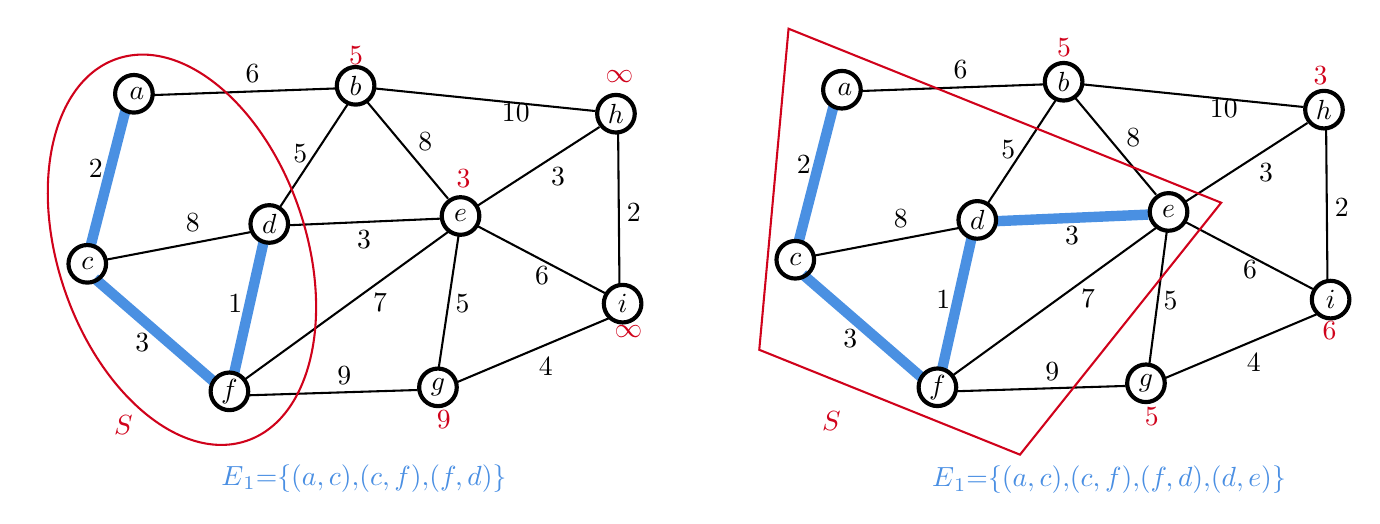
\begin{tikzpicture}[x=0.48pt,y=0.48pt,yscale=-1,xscale=1]
%uncomment if require: \path (0,459); %set diagram left start at 0, and has height of 459

%Straight Lines [id:da6278329343253372] 
\draw [color={rgb, 255:red, 0; green, 0; blue, 0 }  ,draw opacity=1 ][line width=0.75]    (269,67) -- (330,140) ;
%Straight Lines [id:da9826257751124597] 
\draw [color={rgb, 255:red, 0; green, 0; blue, 0 }  ,draw opacity=1 ][line width=0.75]    (179,288) -- (307,284) ;
%Straight Lines [id:da9824647104655378] 
\draw [color={rgb, 255:red, 74; green, 144; blue, 226 }  ,draw opacity=1 ][line width=3.75]    (64,200) -- (154,278) ;
%Straight Lines [id:da5609469664096045] 
\draw [color={rgb, 255:red, 0; green, 0; blue, 0 }  ,draw opacity=1 ][line width=0.75]    (72,186) -- (182,165) ;
%Straight Lines [id:da866584153602073] 
\draw [color={rgb, 255:red, 74; green, 144; blue, 226 }  ,draw opacity=1 ][line width=3.75]    (87,74) -- (61,175) ;
%Straight Lines [id:da8429173178729373] 
\draw [color={rgb, 255:red, 0; green, 0; blue, 0 }  ,draw opacity=1 ][line width=0.75]    (107,62) -- (245,57) ;
%Straight Lines [id:da20128821894816062] 
\draw [color={rgb, 255:red, 0; green, 0; blue, 0 }  ,draw opacity=1 ][line width=0.75]    (255,68) -- (203,147) ;
%Straight Lines [id:da4356587454282608] 
\draw [color={rgb, 255:red, 74; green, 144; blue, 226 }  ,draw opacity=1 ][line width=3.75]    (191,173) -- (169,271) ;
%Straight Lines [id:da14466126019097159] 
\draw [color={rgb, 255:red, 0; green, 0; blue, 0 }  ,draw opacity=1 ][line width=0.75]    (330,165) -- (177,276) ;
%Straight Lines [id:da2637375879467664] 
\draw [color={rgb, 255:red, 0; green, 0; blue, 0 }  ,draw opacity=1 ][line width=0.75]    (324,155) -- (209,160) ;
%Shape: Ellipse [id:dp04172567316274278] 
\draw  [color={rgb, 255:red, 208; green, 2; blue, 27 }  ,draw opacity=1 ] (41.23,208.4) .. controls (14.29,128.98) and (32.03,51.17) .. (80.86,34.61) .. controls (129.7,18.04) and (191.12,68.99) .. (218.07,148.41) .. controls (245.01,227.83) and (227.27,305.64) .. (178.44,322.21) .. controls (129.6,338.78) and (68.18,287.82) .. (41.23,208.4) -- cycle ;
%Straight Lines [id:da22995917519031528] 
\draw [color={rgb, 255:red, 0; green, 0; blue, 0 }  ,draw opacity=1 ][line width=0.75]    (275,57) -- (441,74) ;
%Straight Lines [id:da5296708685106871] 
\draw [color={rgb, 255:red, 0; green, 0; blue, 0 }  ,draw opacity=1 ][line width=0.75]    (458,89) -- (459,204) ;
%Straight Lines [id:da7230804292624167] 
\draw [color={rgb, 255:red, 0; green, 0; blue, 0 }  ,draw opacity=1 ][line width=0.75]    (444,86) -- (351,146) ;
%Straight Lines [id:da9640499330506606] 
\draw [color={rgb, 255:red, 0; green, 0; blue, 0 }  ,draw opacity=1 ][line width=0.75]    (351,160) -- (448,211) ;
%Straight Lines [id:da1957235990181826] 
\draw [color={rgb, 255:red, 0; green, 0; blue, 0 }  ,draw opacity=1 ][line width=0.75]    (451,230) -- (337,278) ;
%Straight Lines [id:da11647241183092005] 
\draw [color={rgb, 255:red, 0; green, 0; blue, 0 }  ,draw opacity=1 ][line width=0.75]    (802,63.94) -- (863,136.94) ;
%Straight Lines [id:da31981297939132225] 
\draw [color={rgb, 255:red, 0; green, 0; blue, 0 }  ,draw opacity=1 ][line width=0.75]    (712,284.94) -- (840,280.94) ;
%Straight Lines [id:da7983678270493085] 
\draw [color={rgb, 255:red, 74; green, 144; blue, 226 }  ,draw opacity=1 ][line width=3.75]    (597,196.94) -- (687,274.94) ;
%Straight Lines [id:da3869238966612649] 
\draw [color={rgb, 255:red, 0; green, 0; blue, 0 }  ,draw opacity=1 ][line width=0.75]    (605,182.94) -- (715,161.94) ;
%Straight Lines [id:da32951243577855704] 
\draw [color={rgb, 255:red, 74; green, 144; blue, 226 }  ,draw opacity=1 ][line width=3.75]    (620,70.94) -- (594,171.94) ;
%Straight Lines [id:da948271107244244] 
\draw [color={rgb, 255:red, 0; green, 0; blue, 0 }  ,draw opacity=1 ][line width=0.75]    (640,58.94) -- (778,53.94) ;
%Straight Lines [id:da9060839913160768] 
\draw [color={rgb, 255:red, 0; green, 0; blue, 0 }  ,draw opacity=1 ][line width=0.75]    (788,64.94) -- (736,143.94) ;
%Straight Lines [id:da54757624583718] 
\draw [color={rgb, 255:red, 74; green, 144; blue, 226 }  ,draw opacity=1 ][line width=3.75]    (724,169.94) -- (702,267.94) ;
%Straight Lines [id:da3064468870257864] 
\draw [color={rgb, 255:red, 0; green, 0; blue, 0 }  ,draw opacity=1 ][line width=0.75]    (863,161.94) -- (710,272.94) ;
%Straight Lines [id:da27846949014065103] 
\draw [color={rgb, 255:red, 74; green, 144; blue, 226 }  ,draw opacity=1 ][line width=3.75]    (857,151.94) -- (742,156.94) ;
%Straight Lines [id:da23340445530829934] 
\draw [color={rgb, 255:red, 0; green, 0; blue, 0 }  ,draw opacity=1 ][line width=0.75]    (808,53.94) -- (974,70.94) ;
%Straight Lines [id:da19179449082275934] 
\draw [color={rgb, 255:red, 0; green, 0; blue, 0 }  ,draw opacity=1 ][line width=0.75]    (991,85.94) -- (992,200.94) ;
%Straight Lines [id:da4737172365295894] 
\draw [color={rgb, 255:red, 0; green, 0; blue, 0 }  ,draw opacity=1 ][line width=0.75]    (977,82.94) -- (884,142.94) ;
%Straight Lines [id:da33516212941033763] 
\draw [color={rgb, 255:red, 0; green, 0; blue, 0 }  ,draw opacity=1 ][line width=0.75]    (884,156.94) -- (981,207.94) ;
%Straight Lines [id:da6079537599641894] 
\draw [color={rgb, 255:red, 0; green, 0; blue, 0 }  ,draw opacity=1 ][line width=0.75]    (984,226.94) -- (870,274.94) ;
%Straight Lines [id:da15519763368476547] 
\draw [color={rgb, 255:red, 0; green, 0; blue, 0 }  ,draw opacity=1 ][line width=0.75]    (338,167) -- (323,267) ;
%Straight Lines [id:da7888476116503551] 
\draw [color={rgb, 255:red, 0; green, 0; blue, 0 }  ,draw opacity=1 ][line width=0.75]    (871,165) -- (858,264) ;
%Shape: Trapezoid [id:dp6408521319989767] 
\draw  [color={rgb, 255:red, 208; green, 2; blue, 27 }  ,draw opacity=1 ] (912,143) -- (760.54,332.67) -- (564.26,253.72) -- (586.31,12.01) -- cycle ;

% Text Node
\draw  [line width=1.5]   (339.38, 153) circle [x radius= 14.15, y radius= 14.15]   ;
\draw (339.38,153) node   [align=left] {$\displaystyle e$};
% Text Node
\draw  [line width=1.5]   (93.48, 61) circle [x radius= 14.15, y radius= 14.15]   ;
\draw (87.98,61) node [anchor=west] [inner sep=0.75pt]   [align=left] {$\displaystyle a$};
% Text Node
\draw  [line width=1.5]   (260.38, 55) circle [x radius= 14.15, y radius= 14.15]   ;
\draw (260.38,55) node   [align=left] {$\displaystyle b$};
% Text Node
\draw  [line width=1.5]   (58.38, 189) circle [x radius= 14.15, y radius= 14.15]   ;
\draw (58.38,189) node   [align=left] {$\displaystyle c$};
% Text Node
\draw  [line width=1.5]   (195.38, 159) circle [x radius= 14.15, y radius= 14.15]   ;
\draw (195.38,159) node   [align=left] {$\displaystyle d$};
% Text Node
\draw  [line width=1.5]   (165.38, 285) circle [x radius= 14.15, y radius= 14.15]   ;
\draw (165.38,285) node   [align=left] {$\displaystyle f$};
% Text Node
\draw  [line width=1.5]   (322.38, 282) circle [x radius= 14.15, y radius= 14.15]   ;
\draw (322.38,282) node   [align=left] {$\displaystyle g$};
% Text Node
\draw (57.24,108.06) node [anchor=north west][inner sep=0.75pt]   [align=left] {$\displaystyle 2$};
% Text Node
\draw (175.24,37.06) node [anchor=north west][inner sep=0.75pt]   [align=left] {$\displaystyle 6$};
% Text Node
\draw (259.24,162.06) node [anchor=north west][inner sep=0.75pt]   [align=left] {$\displaystyle 3$};
% Text Node
\draw (211.24,97.06) node [anchor=north west][inner sep=0.75pt]   [align=left] {$\displaystyle 5$};
% Text Node
\draw (130.24,149.06) node [anchor=north west][inner sep=0.75pt]   [align=left] {$\displaystyle 8$};
% Text Node
\draw (92.24,239.06) node [anchor=north west][inner sep=0.75pt]   [align=left] {$\displaystyle 3$};
% Text Node
\draw (162.24,210.06) node [anchor=north west][inner sep=0.75pt]   [align=left] {$\displaystyle 1$};
% Text Node
\draw (305.24,88.06) node [anchor=north west][inner sep=0.75pt]   [align=left] {$\displaystyle 8$};
% Text Node
\draw (244.24,264.06) node [anchor=north west][inner sep=0.75pt]   [align=left] {$\displaystyle 9$};
% Text Node
\draw (271.24,209) node [anchor=north west][inner sep=0.75pt]   [align=left] {$\displaystyle 7$};
% Text Node
\draw (157,338) node [anchor=north west][inner sep=0.75pt]   [align=left] {$\displaystyle \textcolor[rgb]{0.29,0.56,0.89}{E}\textcolor[rgb]{0.29,0.56,0.89}{_{1}}\textcolor[rgb]{0.29,0.56,0.89}{=}\textcolor[rgb]{0.29,0.56,0.89}{\{}\textcolor[rgb]{0.29,0.56,0.89}{(}\textcolor[rgb]{0.29,0.56,0.89}{a,c}\textcolor[rgb]{0.29,0.56,0.89}{)}\textcolor[rgb]{0.29,0.56,0.89}{,}\textcolor[rgb]{0.29,0.56,0.89}{(}\textcolor[rgb]{0.29,0.56,0.89}{c,f}\textcolor[rgb]{0.29,0.56,0.89}{)}\textcolor[rgb]{0.29,0.56,0.89}{,}\textcolor[rgb]{0.29,0.56,0.89}{(}\textcolor[rgb]{0.29,0.56,0.89}{f,d}\textcolor[rgb]{0.29,0.56,0.89}{)}\textcolor[rgb]{0.29,0.56,0.89}{\}}$};
% Text Node
\draw (76.24,301.06) node [anchor=north west][inner sep=0.75pt]   [align=left] {$\displaystyle \textcolor[rgb]{0.82,0.01,0.11}{S}$};
% Text Node
\draw  [line width=1.5]   (456.38, 76) circle [x radius= 14.15, y radius= 14.15]   ;
\draw (456.38,76) node   [align=left] {$\displaystyle h$};
% Text Node
\draw  [line width=1.5]   (461.38, 219) circle [x radius= 14.15, y radius= 14.15]   ;
\draw (461.38,219) node   [align=left] {$\displaystyle i$};
% Text Node
\draw (393.24,189) node [anchor=north west][inner sep=0.75pt]   [align=left] {$\displaystyle 6$};
% Text Node
\draw (368.24,66) node [anchor=north west][inner sep=0.75pt]   [align=left] {$\displaystyle 10$};
% Text Node
\draw (405.24,114) node [anchor=north west][inner sep=0.75pt]   [align=left] {$\displaystyle 3$};
% Text Node
\draw (462.24,141) node [anchor=north west][inner sep=0.75pt]   [align=left] {$\displaystyle 2$};
% Text Node
\draw (396,257) node [anchor=north west][inner sep=0.75pt]   [align=left] {$\displaystyle 4$};
% Text Node
\draw (253.24,23.06) node [anchor=north west][inner sep=0.75pt]  [color={rgb, 255:red, 208; green, 2; blue, 27 }  ,opacity=1 ] [align=left] {$\displaystyle 5$};
% Text Node
\draw (334,116) node [anchor=north west][inner sep=0.75pt]  [color={rgb, 255:red, 208; green, 2; blue, 27 }  ,opacity=1 ] [align=left] {$\displaystyle 3$};
% Text Node
\draw (319.24,297) node [anchor=north west][inner sep=0.75pt]  [color={rgb, 255:red, 208; green, 2; blue, 27 }  ,opacity=1 ] [align=left] {$\displaystyle 9$};
% Text Node
\draw (453,233) node [anchor=north west][inner sep=0.75pt]  [color={rgb, 255:red, 208; green, 2; blue, 27 }  ,opacity=1 ] [align=left] {$\displaystyle \infty $};
% Text Node
\draw (446.24,41) node [anchor=north west][inner sep=0.75pt]  [color={rgb, 255:red, 208; green, 2; blue, 27 }  ,opacity=1 ] [align=left] {$\displaystyle \infty $};
% Text Node
\draw  [line width=1.5]   (872.38, 149.94) circle [x radius= 14.15, y radius= 14.15]   ;
\draw (872.38,149.94) node   [align=left] {$\displaystyle e$};
% Text Node
\draw  [line width=1.5]   (626.48, 57.94) circle [x radius= 14.15, y radius= 14.15]   ;
\draw (620.98,57.94) node [anchor=west] [inner sep=0.75pt]   [align=left] {$\displaystyle a$};
% Text Node
\draw  [line width=1.5]   (793.38, 51.94) circle [x radius= 14.15, y radius= 14.15]   ;
\draw (793.38,51.94) node   [align=left] {$\displaystyle b$};
% Text Node
\draw  [line width=1.5]   (591.38, 185.94) circle [x radius= 14.15, y radius= 14.15]   ;
\draw (591.38,185.94) node   [align=left] {$\displaystyle c$};
% Text Node
\draw  [line width=1.5]   (728.38, 155.94) circle [x radius= 14.15, y radius= 14.15]   ;
\draw (728.38,155.94) node   [align=left] {$\displaystyle d$};
% Text Node
\draw  [line width=1.5]   (698.38, 281.94) circle [x radius= 14.15, y radius= 14.15]   ;
\draw (698.38,281.94) node   [align=left] {$\displaystyle f$};
% Text Node
\draw  [line width=1.5]   (855.38, 278.94) circle [x radius= 14.15, y radius= 14.15]   ;
\draw (855.38,278.94) node   [align=left] {$\displaystyle g$};
% Text Node
\draw (590.24,105) node [anchor=north west][inner sep=0.75pt]   [align=left] {$\displaystyle 2$};
% Text Node
\draw (708.24,34) node [anchor=north west][inner sep=0.75pt]   [align=left] {$\displaystyle 6$};
% Text Node
\draw (792.24,159) node [anchor=north west][inner sep=0.75pt]   [align=left] {$\displaystyle 3$};
% Text Node
\draw (744.24,94) node [anchor=north west][inner sep=0.75pt]   [align=left] {$\displaystyle 5$};
% Text Node
\draw (663.24,146) node [anchor=north west][inner sep=0.75pt]   [align=left] {$\displaystyle 8$};
% Text Node
\draw (625.24,236) node [anchor=north west][inner sep=0.75pt]   [align=left] {$\displaystyle 3$};
% Text Node
\draw (695.24,207) node [anchor=north west][inner sep=0.75pt]   [align=left] {$\displaystyle 1$};
% Text Node
\draw (838.24,85) node [anchor=north west][inner sep=0.75pt]   [align=left] {$\displaystyle 8$};
% Text Node
\draw (777.24,261) node [anchor=north west][inner sep=0.75pt]   [align=left] {$\displaystyle 9$};
% Text Node
\draw (804.24,205.94) node [anchor=north west][inner sep=0.75pt]   [align=left] {$\displaystyle 7$};
% Text Node
\draw (692,338.94) node [anchor=north west][inner sep=0.75pt]   [align=left] {$\displaystyle \textcolor[rgb]{0.29,0.56,0.89}{E}\textcolor[rgb]{0.29,0.56,0.89}{_{1}}\textcolor[rgb]{0.29,0.56,0.89}{=}\textcolor[rgb]{0.29,0.56,0.89}{\{}\textcolor[rgb]{0.29,0.56,0.89}{(}\textcolor[rgb]{0.29,0.56,0.89}{a,c}\textcolor[rgb]{0.29,0.56,0.89}{)}\textcolor[rgb]{0.29,0.56,0.89}{,}\textcolor[rgb]{0.29,0.56,0.89}{(}\textcolor[rgb]{0.29,0.56,0.89}{c,f}\textcolor[rgb]{0.29,0.56,0.89}{)}\textcolor[rgb]{0.29,0.56,0.89}{,}\textcolor[rgb]{0.29,0.56,0.89}{(}\textcolor[rgb]{0.29,0.56,0.89}{f,d}\textcolor[rgb]{0.29,0.56,0.89}{) ,}\textcolor[rgb]{0.29,0.56,0.89}{( d,e)\}}$};
% Text Node
\draw (609.24,298) node [anchor=north west][inner sep=0.75pt]   [align=left] {$\displaystyle \textcolor[rgb]{0.82,0.01,0.11}{S}$};
% Text Node
\draw  [line width=1.5]   (989.38, 72.94) circle [x radius= 14.15, y radius= 14.15]   ;
\draw (989.38,72.94) node   [align=left] {$\displaystyle h$};
% Text Node
\draw  [line width=1.5]   (994.38, 215.94) circle [x radius= 14.15, y radius= 14.15]   ;
\draw (994.38,215.94) node   [align=left] {$\displaystyle i$};
% Text Node
\draw (926.24,183.94) node [anchor=north west][inner sep=0.75pt]   [align=left] {$\displaystyle 6$};
% Text Node
\draw (901.24,62.94) node [anchor=north west][inner sep=0.75pt]   [align=left] {$\displaystyle 10$};
% Text Node
\draw (938.24,110.94) node [anchor=north west][inner sep=0.75pt]   [align=left] {$\displaystyle 3$};
% Text Node
\draw (995.24,137.94) node [anchor=north west][inner sep=0.75pt]   [align=left] {$\displaystyle 2$};
% Text Node
\draw (929,253.94) node [anchor=north west][inner sep=0.75pt]   [align=left] {$\displaystyle 4$};
% Text Node
\draw (786.24,17) node [anchor=north west][inner sep=0.75pt]  [color={rgb, 255:red, 208; green, 2; blue, 27 }  ,opacity=1 ] [align=left] {$\displaystyle 5$};
% Text Node
\draw (852.24,294.94) node [anchor=north west][inner sep=0.75pt]  [color={rgb, 255:red, 208; green, 2; blue, 27 }  ,opacity=1 ] [align=left] {$\displaystyle 5$};
% Text Node
\draw (986,229.94) node [anchor=north west][inner sep=0.75pt]  [color={rgb, 255:red, 208; green, 2; blue, 27 }  ,opacity=1 ] [align=left] {$\displaystyle 6$};
% Text Node
\draw (979.24,37.94) node [anchor=north west][inner sep=0.75pt]  [color={rgb, 255:red, 208; green, 2; blue, 27 }  ,opacity=1 ] [align=left] {$\displaystyle 3$};
% Text Node
\draw (866.24,207.94) node [anchor=north west][inner sep=0.75pt]   [align=left] {$\displaystyle 5$};
% Text Node
\draw (333.24,209.94) node [anchor=north west][inner sep=0.75pt]   [align=left] {$\displaystyle 5$};


\end{tikzpicture}

